\section{Introduction} \label{intro}

So far, the Standard Model (SM) of particle physics is the most successful theory to describe fundamental particles and their interactions. It is a renormalizable, chiral, gauge quantum field theory (QFT) defined by the local SU(3)$_C \times$SU(2)$_L\times$U(1)$_Y$ gauge symmetry that describes the strong and electroweak forces.  The unification of the electromagnetic and weak forces leading to the electroweak force was experimentally verified by the discovery of the $Z$ boson in 1983 at the Super Proton Synchrotron (SPS) at CERN \cite{Zboson}. Nevertheless, although in this theory the gauge bosons $W^\pm$ and $Z$ are considered to be massless, the experimental results proved the opposite. To explain the mass of these particles, the Higgs field is introduced in the SM by adding the Higgs potential to the SM lagrangian (Figure \ref{fig: Higgs portential}).

The Higgs field is an electrically neutral scalar field symmetric under the SM gauge symmetries. Nevertheless, it has an infinite number of ground states and any given ground state is not invariant under the U(1)$_Y$ nor SU(2)$_L$ groups but is symmetric under U(1)$_Q$, with $Q$ being the electric charge. This leads to the Electroweak Symmetry Breaking (EWSB) of the SM. Therefore, the SU(3)$_C \times$SU(2)$_L\times$U(1)$_Y$ gauge group is spontaneously broken to SU(3)$_C \times$U(1)$_Q$ \cite{EWSB}. The Brout–Englert–Higgs mechanism explains this spontaneous symmetry breaking via which the $W\pm$ and $Z$ gauge bosons can acquire mass. \cite{Higgs64}

\begin{figure}[hbt]
    \centering
    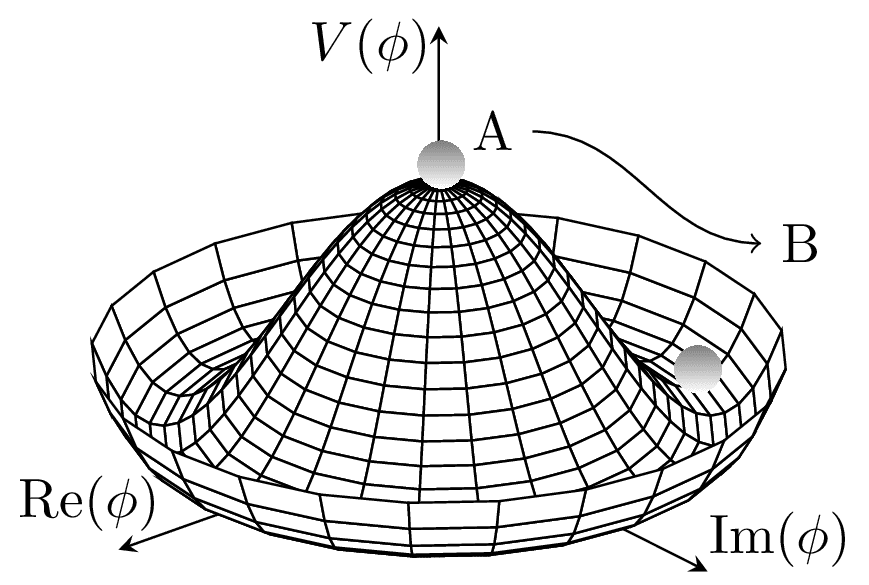
\includegraphics[width=0.4\linewidth]{Images/1.Intro/higgs-potential.png}
    \caption{Shape of the Higgs potential V($\Phi$). The spontaneous symmetry breaking is observed as a particle in this field goes from point A to a given ground state at point B that is not invariant under the SM gauge symmetries. \cite{HiggsPotdrawing}}
    \label{fig: Higgs portential}
\end{figure}

The Higgs boson is an excitation of the Higgs field and its discovery by the ATLAS \cite{ATLASdecouvhiggs} and CMS \cite{CMShiggsdecouv} experiments in 2012 proves the existence of a fundamental scalar sector in the SM. The Higgs boson mass measured by the CMS experiment is 125.38 GeV with a precision of 0.14 GeV \cite{PreciseCMSmeasHiggs}. To further characterize this particle, there is an ongoing experimental effort to determine the value of the Higgs self-coupling constant $\lambda$, which will also allow to probe the shape of the scalar potential of the Higgs, that is governed by this parameter. This will be described in more detail in Section \ref{section: HH4b}. In order to probe the value of this self-coupling constant $\lambda$, the di-Higgs (HH) production is studied. In this thesis, SPANet \cite{SPANet}, an attention-based neural network is introduced for the HH $\to$ 4b analysis that aims to constrain the value of $\lambda$. 

The thesis is structured as follows. Section \ref{section: CMS} gives a short overview of the Large Hadron Collider (LHC) and the Compact Muon Solenoid (CMS) experiment. Section \ref{section: HH4b} delves into some theoretical and experimental aspects of the HH $\to$ 4b analysis. Section \ref{section: spanet architecture} introduces some concepts of Machine Learning and presents the neural network proposed to be employed in the HH $\to$ 4b analysis: SPANet. Section \ref{section: improving} presents the results of the pairing between the reconstructed jets and generator-level quarks using SPANet. Section \ref{section: s/b classification} presents the results of the signal/background (S/B) classification for the HH $\to$ 4b analysis using SPANet as classifier. Finally, Section \ref{section: conclusion} summarizes the obtained results and provides a short outlook on the next steps.

% Explain better the Higgs flied and the potential and so on. The Higgs boson is excitation of this field. It's discovery proves the existence of a fundamental scalar sector in the SM.

%Nowadays the Higgs boson mass measured by the CMS experiment is 125.53 GeV with a precision of 0.15 GeV (cite). To further characterize this particle, there is an ongoing experimental effort to determine the value of the self-coupling $\lambda$, which will also allow to probe the shape of the scalar potential of the Higgs mechanism.

%brief intro on renorm QFT and symmetries